\documentclass{beamer}

\usepackage[utf8]{inputenc}
\usepackage[T2A]{fontenc}
\usepackage[russian]{babel}

\usepackage{url}
\usepackage{qrcode}

\usepackage{amsmath}
\usepackage{tikz}
\usepackage{graphicx}
\usepackage{svg}
\usepackage{wrapfig}

\usetheme{Madrid}

\defbeamertemplate*{title page}{customized}[1][]
{
    \begin{center}
        \usebeamerfont{title}
        \inserttitle
        \par
    \end{center}
    \bigskip
    \hfill
    \hbox{
        \usebeamerfont{author}
        \begin{tabular}{ll}
            Студент: & Суркис Антон Игоревич \\
            Научный руководитель: & Попов Иван Александрович \\
        \end{tabular}
    }
    \par
    \begin{center}
        \usebeamerfont{date}
        Университет ИТМО
        \par
        \insertdate
        \par
    \end{center}
}

\title[Ограничения Nanite]{Исследование ограничений процедурного кластерного видозависимого лоддирования в современных компьютерных играх}
\author{Антон Суркис}

\begin{document}
    \maketitle
    \begin{frame}{Введение}
    \begin{itemize}
        \item В современных компьютерных играх для реалистичной графики используют высокодетализированные модели объектов
        \item Отрисовывать все детали всех объектов на экране очень долго
        \item Классическое решение --- монолитная детализация, Level of Detail (LOD, лод)
        \item Лоды создаются вручную, это дорого
        \item Лоды сложно применять на больших объектах (зданиях, скалах)
    \end{itemize}
    \begin{center}
        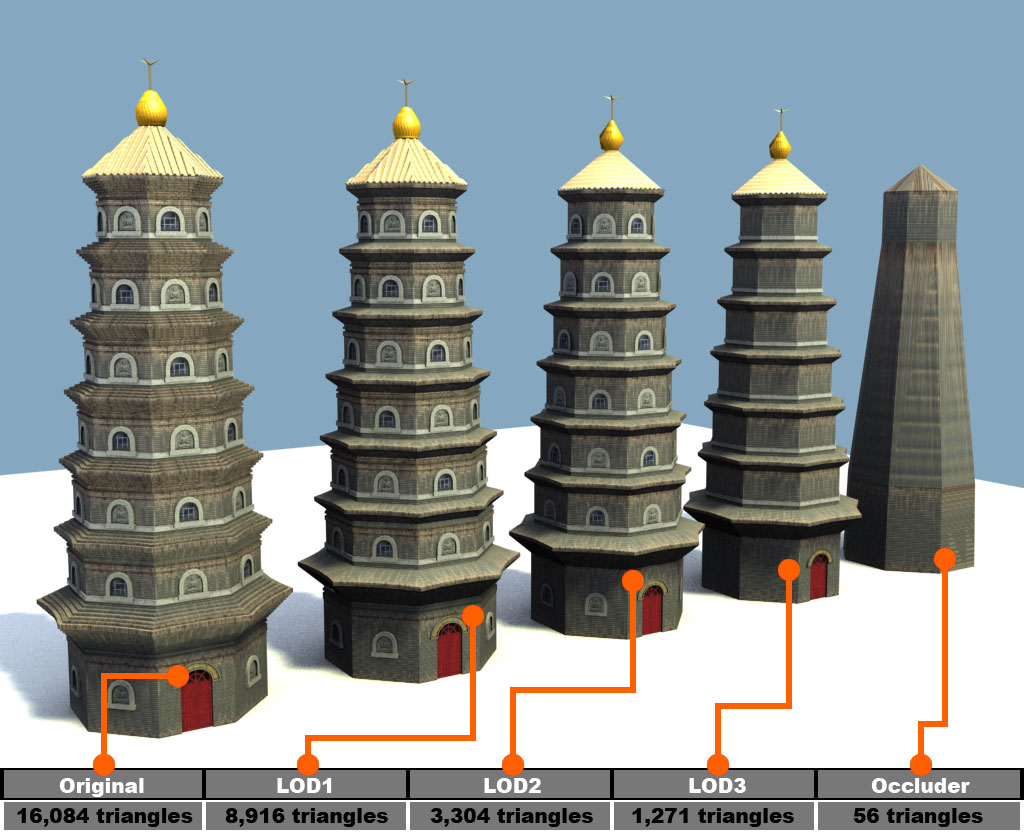
\includegraphics[height=.4\textheight]{pics/lod.jpg}
    \end{center}
\end{frame}

\begin{frame}{Альтернативы лодам}
    \begin{itemize}
        \item Geometry Clipmaps\footnote{GPU Gems 2, глава 2} --- только для ландшафта
        \item Sparse Voxel Octrees\footnote{\url{https://research.nvidia.com/sites/default/files/pubs/2010-02_Efficient-Sparse-Voxel/laine2010tr1_paper.pdf}} --- неточен, требует много памяти
        \item Nanite от Epic Games --- лучшее известное решение:
        \begin{itemize}
            \item Не нужна ручная обработка
            \item Хорошо работает на больших объектах
            \item Максимальная детализация, на которую хватает разрешения экрана
        \end{itemize}

        \alert{Но за 4 года никто другой не достиг подобных результатов с подобной технологией}
    \end{itemize}
\end{frame}

\begin{frame}{Цели и задачи}
    \textbf{Цель работы:}
    продемонстрировать работоспособность технологии процедурного кластерного видозависимого лоддирования и определить её ограничения

    \bigskip

    \textbf{Задачи:}
    \begin{itemize}
        \item Изучить механизм работы Nanite
        \item Реализовать упрощённую систему процедурного кластерного видозависимого изменения детализации
        \item Определить проблемы, возникающие при реализации
        \item Определить принципиальные ограничения технологии
        \item Сравнить с монолитной детализацией
    \end{itemize}
\end{frame}

    \begin{frame}{Nanite}
    \begin{itemize}
        \item Меш --- набор треугольников, мешлет --- ограниченный по размеру меш
        \item Nanite преобразует меш в направленный ациклический граф мешлетов
        \item Стоки --- разбиение исходного меша
        \item Вершины следующего уровня --- лоды объединений вершин предыдущего уровня
        \item Отрисовываются мешлеты в разрезе графа
        \item Свойство графа: из вершины графа за $O(1)$ определяется, входит ли она в разрез
    \end{itemize}
    \begin{center}
        \includesvg[width=.45\textwidth]{nanite-dag.svg}
        \includesvg[width=.45\textwidth]{nanite-dag-cut.svg}
    \end{center}
\end{frame}

\begin{frame}{Nanite: пример предподсчёта, шаг 1}
    \centering \includesvg{meshlets-0.svg}
\end{frame}

\begin{frame}{Nanite: пример предподсчёта, шаг 2}
    \centering \includesvg{meshlets-1.svg}
\end{frame}

\begin{frame}{Nanite: пример предподсчёта, шаг 3}
    \centering \includesvg{meshlets-2.svg}
\end{frame}

\begin{frame}{Nanite: пример предподсчёта, шаг 4}
    \centering \includesvg{meshlets-3.svg}
\end{frame}

    \clearpage
\section{2 РЕАЛИЗАЦИЯ УПРОЩЁННОЙ СИСТЕМЫ}
Реализация упрощённой системы проводилась параллельно с изучением работы Nanite и нужна для лучшего понимания механизма работы Nanite, а также для выявления его технических и принципиальных ограничений.

Было решено отказаться от реализации параллельного спуска по графу и специального механизма отрисовки треугольников размером менее четырёх пикселей, а также от текстурирования.
Ожидается, что эти части не покажут принципиальных ограничений технологии.

Предподсчёт и непосредственно отрисовку было решено сделать в виде разных приложений, результат предподсчёта сериализуется на диск.

\subsection*{Предподсчёт}
При реализации первого шага предподсчёта было определено существенное ограничение библиотеки METIS --- она не поддерживает задание жёсткого ограничения на размер сегмента, только конечный штраф за неравномерность размеров.
Для того, чтобы не превысить размер мешлета, было решено задавать большее количество мешлетов, чем идеальное, изучение исходного кода Nanite показало, что в нём используется то же решение~\cite{NaniteSrcMETIS}.

При объединении стоков графа в группы было обнаружено, что объединить их ровно по 4 оказалось также невозможно, поэтому было принято решение использовать примерное объединение по 4 в среднем.

Определение швов основывалось на предположении, что на каждой итерации цикла стоки графа мешлетов образуют поверхность замкнутого объёма.
В противном случае возможно подобрать ракурс и порог так, чтобы нарушить свойство графа об отсутствии щелей.
Тогда каждое ребро, находящееся целиком внутри супермешлета, принадлежит ровно двум треугольникам этого супермешлета, остальные рёбра считаются частью шва.

Для децимации были использованы два алгоритма:
\begin{itemize}
    \item тривиальный алгоритм, схлопывающий рёбра, не лежащие на шве, без учёта добавленного искажения.
    Этот алгоритм был использован на ранних этапах разработки для проверки корректности определения швов;
    \item Decimation with Error Quadrics~\cite{DecimationQuadrics}, который наиболее часто используется при децимации для стандартного подхода к уровням детализации и даёт высокую точность результата.
    Этот алгоритм был использован в финальной версии.
\end{itemize}

Разбиение децимированного супермешлета производилось аналогично первому шагу предподсчёта, но не всегда строго на 2 мешлета --- в некоторых случаях степени децимации было недостаточно, поэтому количество мешлетов при разбиении было подстроено, чтобы мешлеты не превышали ограничение по размеру.

В некоторых случаях из-за этого итерации цикла не уменьшали количество стоков, а длились бесконечно.
Из-за этого было принято решение добавить ещё одно условие к остановке цикла --- если итерация не уменьшила количество стоков, то цикл завершается.

Граф сохраняется как массив мешлетов, массив вершин, массив индексов и массив примитивов.

Запись мешлета представляет собой количество вершин в мешлете, начало мешлета в массиве индексов, количество примитивов в мешлете, начало мешлета в массиве примитивов, количество родителей этого мешлета и номер первого родителя в массиве мешлетов.

Массив вершин хранит позицию и нормаль вершины.

Массив индексов состоит из идущих подряд без разделителей срезов, каждый из которых соответствует одному мешлету.
Срез содержит неповторяющиеся индексы тех вершин, которые входят в мешлет.
Старший бит индекса используется для записи, входит ли эта вершина в шов мешлета.

Массив примитивов состоит из идущих подряд без разделителей срезов, каждый из которых соответствует одному мешлету.
Срез содержит индексы элементов в соответствующем срезе в массиве индексов, и упакован в 10 битов на компонент, один элемент среза --- 32-битное целое число.

\subsection*{Отрисовка}
\subsubsection*{Используемые технологии}
Для реализации приложения, выполняющего отрисовку графа, было решено использовать API DirectX~12.
Главными факторами в этом решении стали поддержка технологии Mesh Shader, позволяющей отправлять на отрисовку наборы мешлетов, и поддержка средства отладки графики PIX~\cite{PIX}.

Также возможно было бы использовать API Vulkan с расширением \\
\texttt{VK\_EXT\_mesh\_shader}, но проект DirectX~12 оказался проще в настройке.
Также основной инструмент отладки для Vulkan --- RenderDoc --- не поддерживал Mesh Shader на момент написания работы, в отличие от PIX.

Более простой в использовании DirectX~11 не поддерживает технологию Mesh Shader.

Более простой в использовании OpenGL~4 поддерживает Mesh Shader в виде расширения NVidia \texttt{GL\_NV\_mesh\_shader}, но его основным инструментом отладки, также как и для Vulkan, является RenderDoc.

Поддержка Mesh Shader не является необходимой для процедурного кластерного видозависимого лоддирования, поскольку отрисовку мешлетов можно реализовать с помощью классического конвейера, но преимущество в производительности предполагается только при её использовании, поэтому в рамках работы было решено реализовывать отрисовку мешлетов только через Mesh Shader.

Упрощённое описание работы классического конвейера:
\begin{enumerate}
    \item устанавливается массив вершин, массив индексов вершин, формат примитивов, описанных в массиве индексов вершин (точки, независимые отрезки, ломаная линия, треугольники, и т.д.);
    \item для примитивов выбираются вершины из массива вершин и преобразовываются с помощью вершинного шейдера.
    Вершинный шейдер выполняет преобразования над одной вершиной --- он не может убирать или добавлять вершины.
    Обычно его работа заключается в определении положения вершины в проективном пространстве;
    \item вершины проецируются на экран, определяются пиксели для растеризации примитивов.
    Механизм проекцикци и растеризации --- непрограммируемый;
    \item для каждого растеризуемого пикселя запускается пиксельный шейдер, ему на вход подаётся интерполяция вершин примитива, которому принадлежит этот пиксель.
    Пиксельный шейдер определяет конечный цвет пикселя в виде четырёхмерного вектора вещественных чисел --- три компоненты задают красную, зелёную и синюю составляющие цвета, четвёртая задаёт коэффициент смешивания с предыдущим цветом этого пикселя на экране.
\end{enumerate}

Упрощённое описание работы Mesh Shader:
\begin{enumerate}
    \item устанавливается количество групп потоков для шейдера расширения (Amplification Shader);
    \item каждая группа потоков шейдера расширения приходит к консенсусу о количестве групп потоков шейдеров сетки (Mesh Shader) и дополнительной информации, одинаковой для каждого потока.
    Группы потоков шейдеров сетки от разных групп потоков шейдеров расширения независимы друг от друга, например, если первая группа потоков шейдеров расширения примет решение запустить 5 групп потоков шейдеров сетки, а вторая --- 6, то всего будет запущено 11 групп потоков шейдеров сетки.
    Консенсус потоков шейдеров расширения внутри одной группы должен быть доказан компилятором.
    Каждому потоку известен его номер в группе и номер его группы, что позволяет ему прочитать из видеопамяти остальные данные, которые он должен обработать;

    \item каждая группа потоков шейдеров сетки задаёт один мешлет: на этапе компиляции определяется максимально возможное количество вершин и примитивов в одном мешлете, а также тип примитива --- точка, отрезок или треугольник.
    Группа потоков шейдеров сетки приходит к консенсусу о количестве вершин и примитивов мешлета и записывает в общую память группы потоков информацию о вершинах и примитивах.
    Консенсус количества вершин и примитивов должен быть доказан компилятором.

    Тип вершины является структурой с помеченными полями, тип примитива --- беззнаковое целое число для точки, вектор из двух беззнаковых целых чисел для отрезка или вектор из трёх беззнаковых целых чисел для треугольника.

    Тип вершины обязательно должен содержать четырёхмерный вектор вещественных чисел, помеченный выделенной меткой, этот вектор обозначает позицию вершины в проективном трёхмерном пространстве.

    Значение примитива --- это индексы в записанном массиве вершин, это позволяет уменьшить использование памяти для тех вершин, которые повторяются в нескольких примитивах.
    В наиболее распространённом случае, когда меш описывает поверхность замкнутого объёма, а мешлет является связным фрагментом меша, таких повторяющихся вершин --- подавляющее большинство;

    \item вершины проецируются на экран, определяются пиксели для растеризации примитивов.
    Механизм проекции и растеризации --- непрограммируемый;

    \item для каждого растеризуемого пикселя запускается пиксельный шейдер, ему на вход подаётся интерполяция вершин примитива, которому принадлежит этот пиксель.
    Пиксельный шейдер определяет конечный цвет пикселя в виде четырёхмерного вектора вещественных чисел --- три компоненты задают красную, зелёную и синюю составляющие цвета, четвёртая задаёт коэффициент смешивания с предыдущим цветом этого пикселя на экране.
    В отличие от шейдера расширения и шейдера сетки, пиксельный шейдер не имеет информации о потоке и группе потоков, ему известны только интерполированная вершина и абсолютные координаты пикселя на экране.
\end{enumerate}

\subsubsection*{Детали реализации}
При десериализации данных массив вершин преобразовывается так, чтобы шейдер сетки не обращался к массиву индексов, а непосредственно брал поряд идущие вершины сразу из массива.
О причинах этого решения --- в главе~5.

В упрощённой реализации процедурного кластерного видозависимого лоддирования шейдеры работают следующим образом:
\begin{itemize}
    \item количество групп потоков шейдера расширения определяется таким, чтобы каждому мешлету в графе соответствовал один поток шейдера расширения;
    \item один поток шейдера расширения определяет, должен ли быть отрисован соответствующий ему мешлет.
    Для этого он определяет, подходит ли этот мешлет по точности и пересекает ли описывающий объём этого мешлета область видимости;
    \item потоки шейдера расширения внутри одной группы упорядочивают мешлеты, подходящие для отрисовки, чтобы они образовали сплошной массив в общей для группы потоков памяти, количество групп мешлетов задаётся равным длине этого массива, а сам массив устанавливается как дополнительная информация для шейдера сетки;
    \item поток шейдера сетки, исходя из полученного массива, копирует информацию о вершинах и примитивах из глобального буфера, добавляя в вершины информацию о номере мешлета;
    \item пиксельный шейдер окрашивает пиксели в цвет мешлета соответственно палитре.
    Это существенно помогает при отладке.
\end{itemize}

Для оценки искажения расположение мешлета приближается с помощью описывающего прямоугольного параллелепипеда со сторонами, параллельными осям координат.
Такие прямоугольные параллелепипеды обозначаются английской аббревиатурой AABB --- Axis-Aligned Bounding Box.
Для записи AABB достаточно двух трёхмерных векторов --- минимальные и максимальные координаты по всем трём осям.

Можно заметить, что AABB меша не зависит от порядка обхода примитивов и вершин, принадлежащих этим примитивам.

На рисунке~\ref{fig:AABB} приведён AABB (обозначен красным) для двумерной фигуры (обозначена синим).

\begin{figure}[ht]
    \centering
    \begin{tikzpicture}
        \filldraw[fill=blue!25] (1,1) -- (5,2) -- (4, 4) -- (3,2) -- (1,5) -- (2,2) -- (1,1);
        \draw[thick,red] (1,1) rectangle (5,5);
        \draw[thick,->,>=stealth] (-1,0) -- (6,0);
        \draw[thick,->,>=stealth] (0,-1) -- (0,6);
    \end{tikzpicture}
    \caption{Двумерный пример AABB}
    \label{fig:AABB}
\end{figure}

Для отладки как предподсчёта, так и самой отрисовки, в приложение был добавлен простой пользовательский интерфейс с помощью библиотеки imgui.
Интерфейс предоставляет настройки отрисовки самих мешлетов, их AABB, выбора порога точности и выбора режима отображения мешлетов.
Существующие режимы отображения:
\begin{itemize}
    \item отрисовка мешлетов с учётом оценки искажения;
    \item отрисовка мешлетов определённого слоя.
    Здесь и далее слоем называется набор стоков графа мешлетов, существовавший на определённой итерации;
    \item отрисовка мешлетов определённого слоя с покраской, показывающей, в какие супермешлеты они были объединены;
    \item отрисовка мешлетов определённого слоя с отображением чёрным тех вершин, которые входят в шов.
\end{itemize}

На рисунке~\ref{fig:execution-example} приведён пример выполнения программы.
Исходная модель содержит 10 млн. треугольников и 4~999~996 вершин, для 64 копий модели (не все из которых видны в кадре) отправляется на отрисовку 11~307~215 треугольников.

\begin{figure}[ht]
    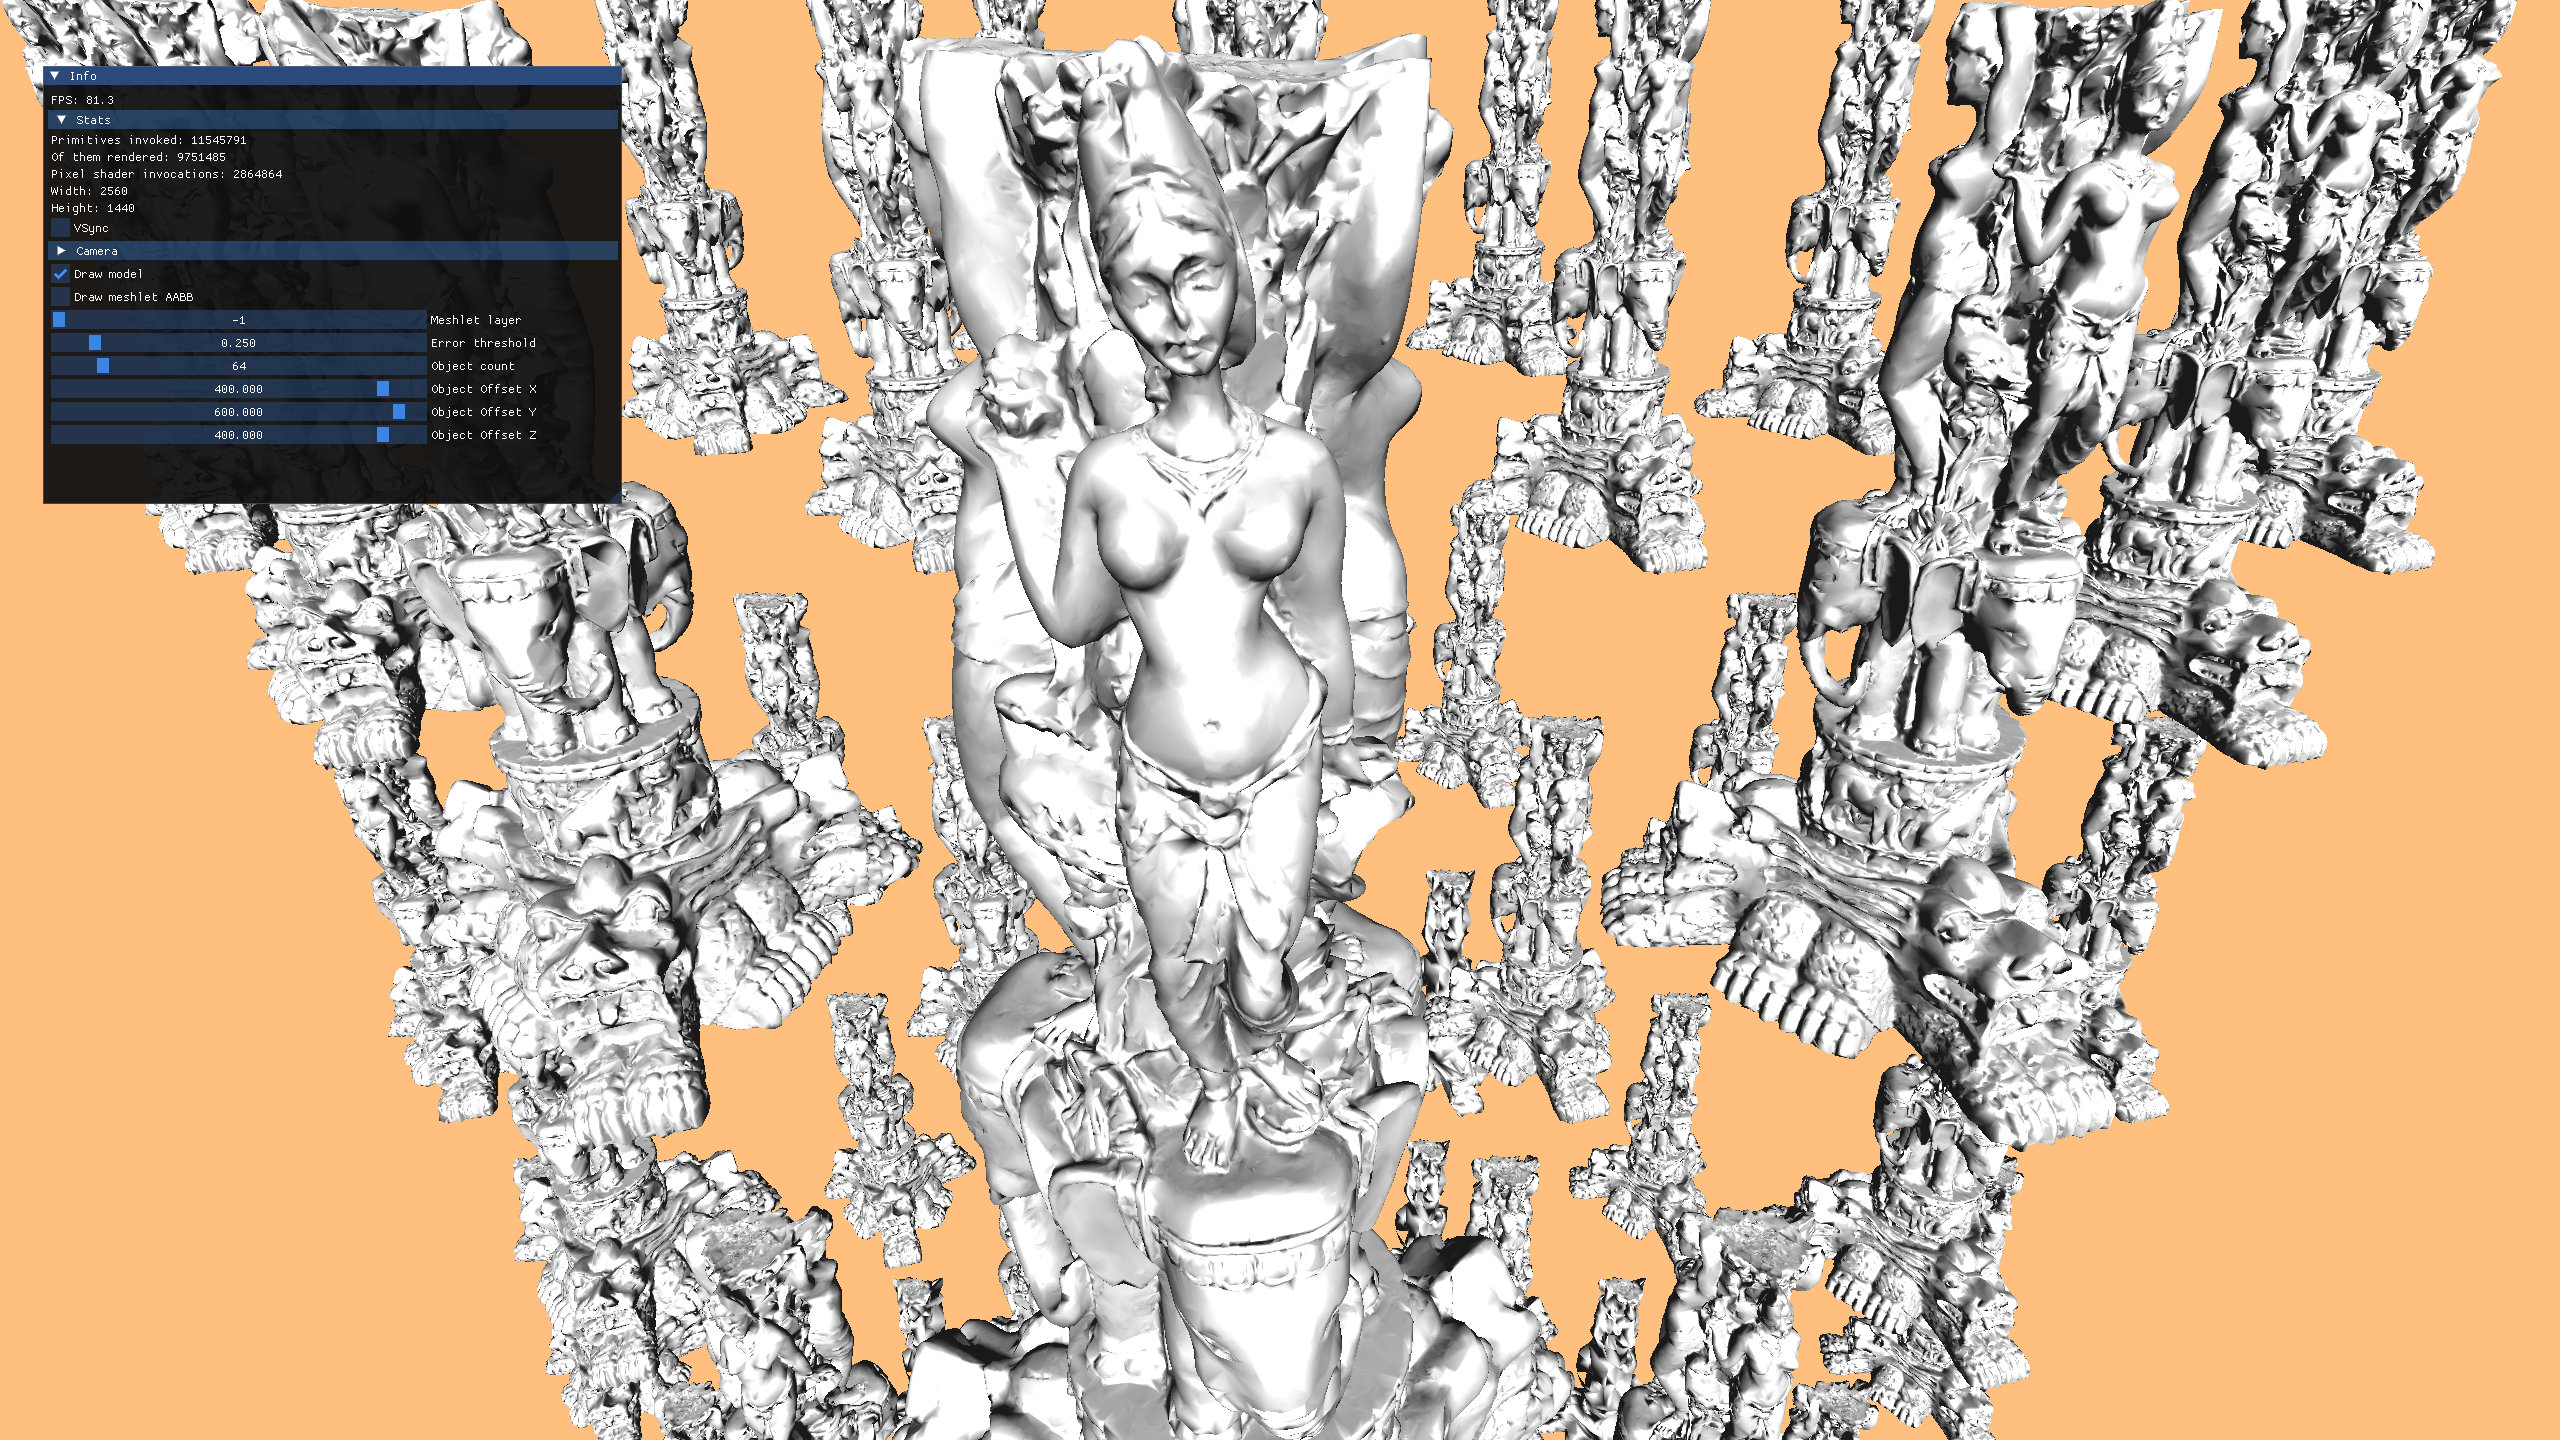
\includegraphics[width=\textwidth]{pics/impl2.png}
    \caption{Выполнение}
    \label{fig:execution-example}
\end{figure}

На рисунке~\ref{fig:impl-example} приведены примеры отрисовки программой одного и того же объекта на разном удалении от камеры.

\begin{figure}[ht]
    \centering

    \begin{subfigure}{.45\textwidth}
        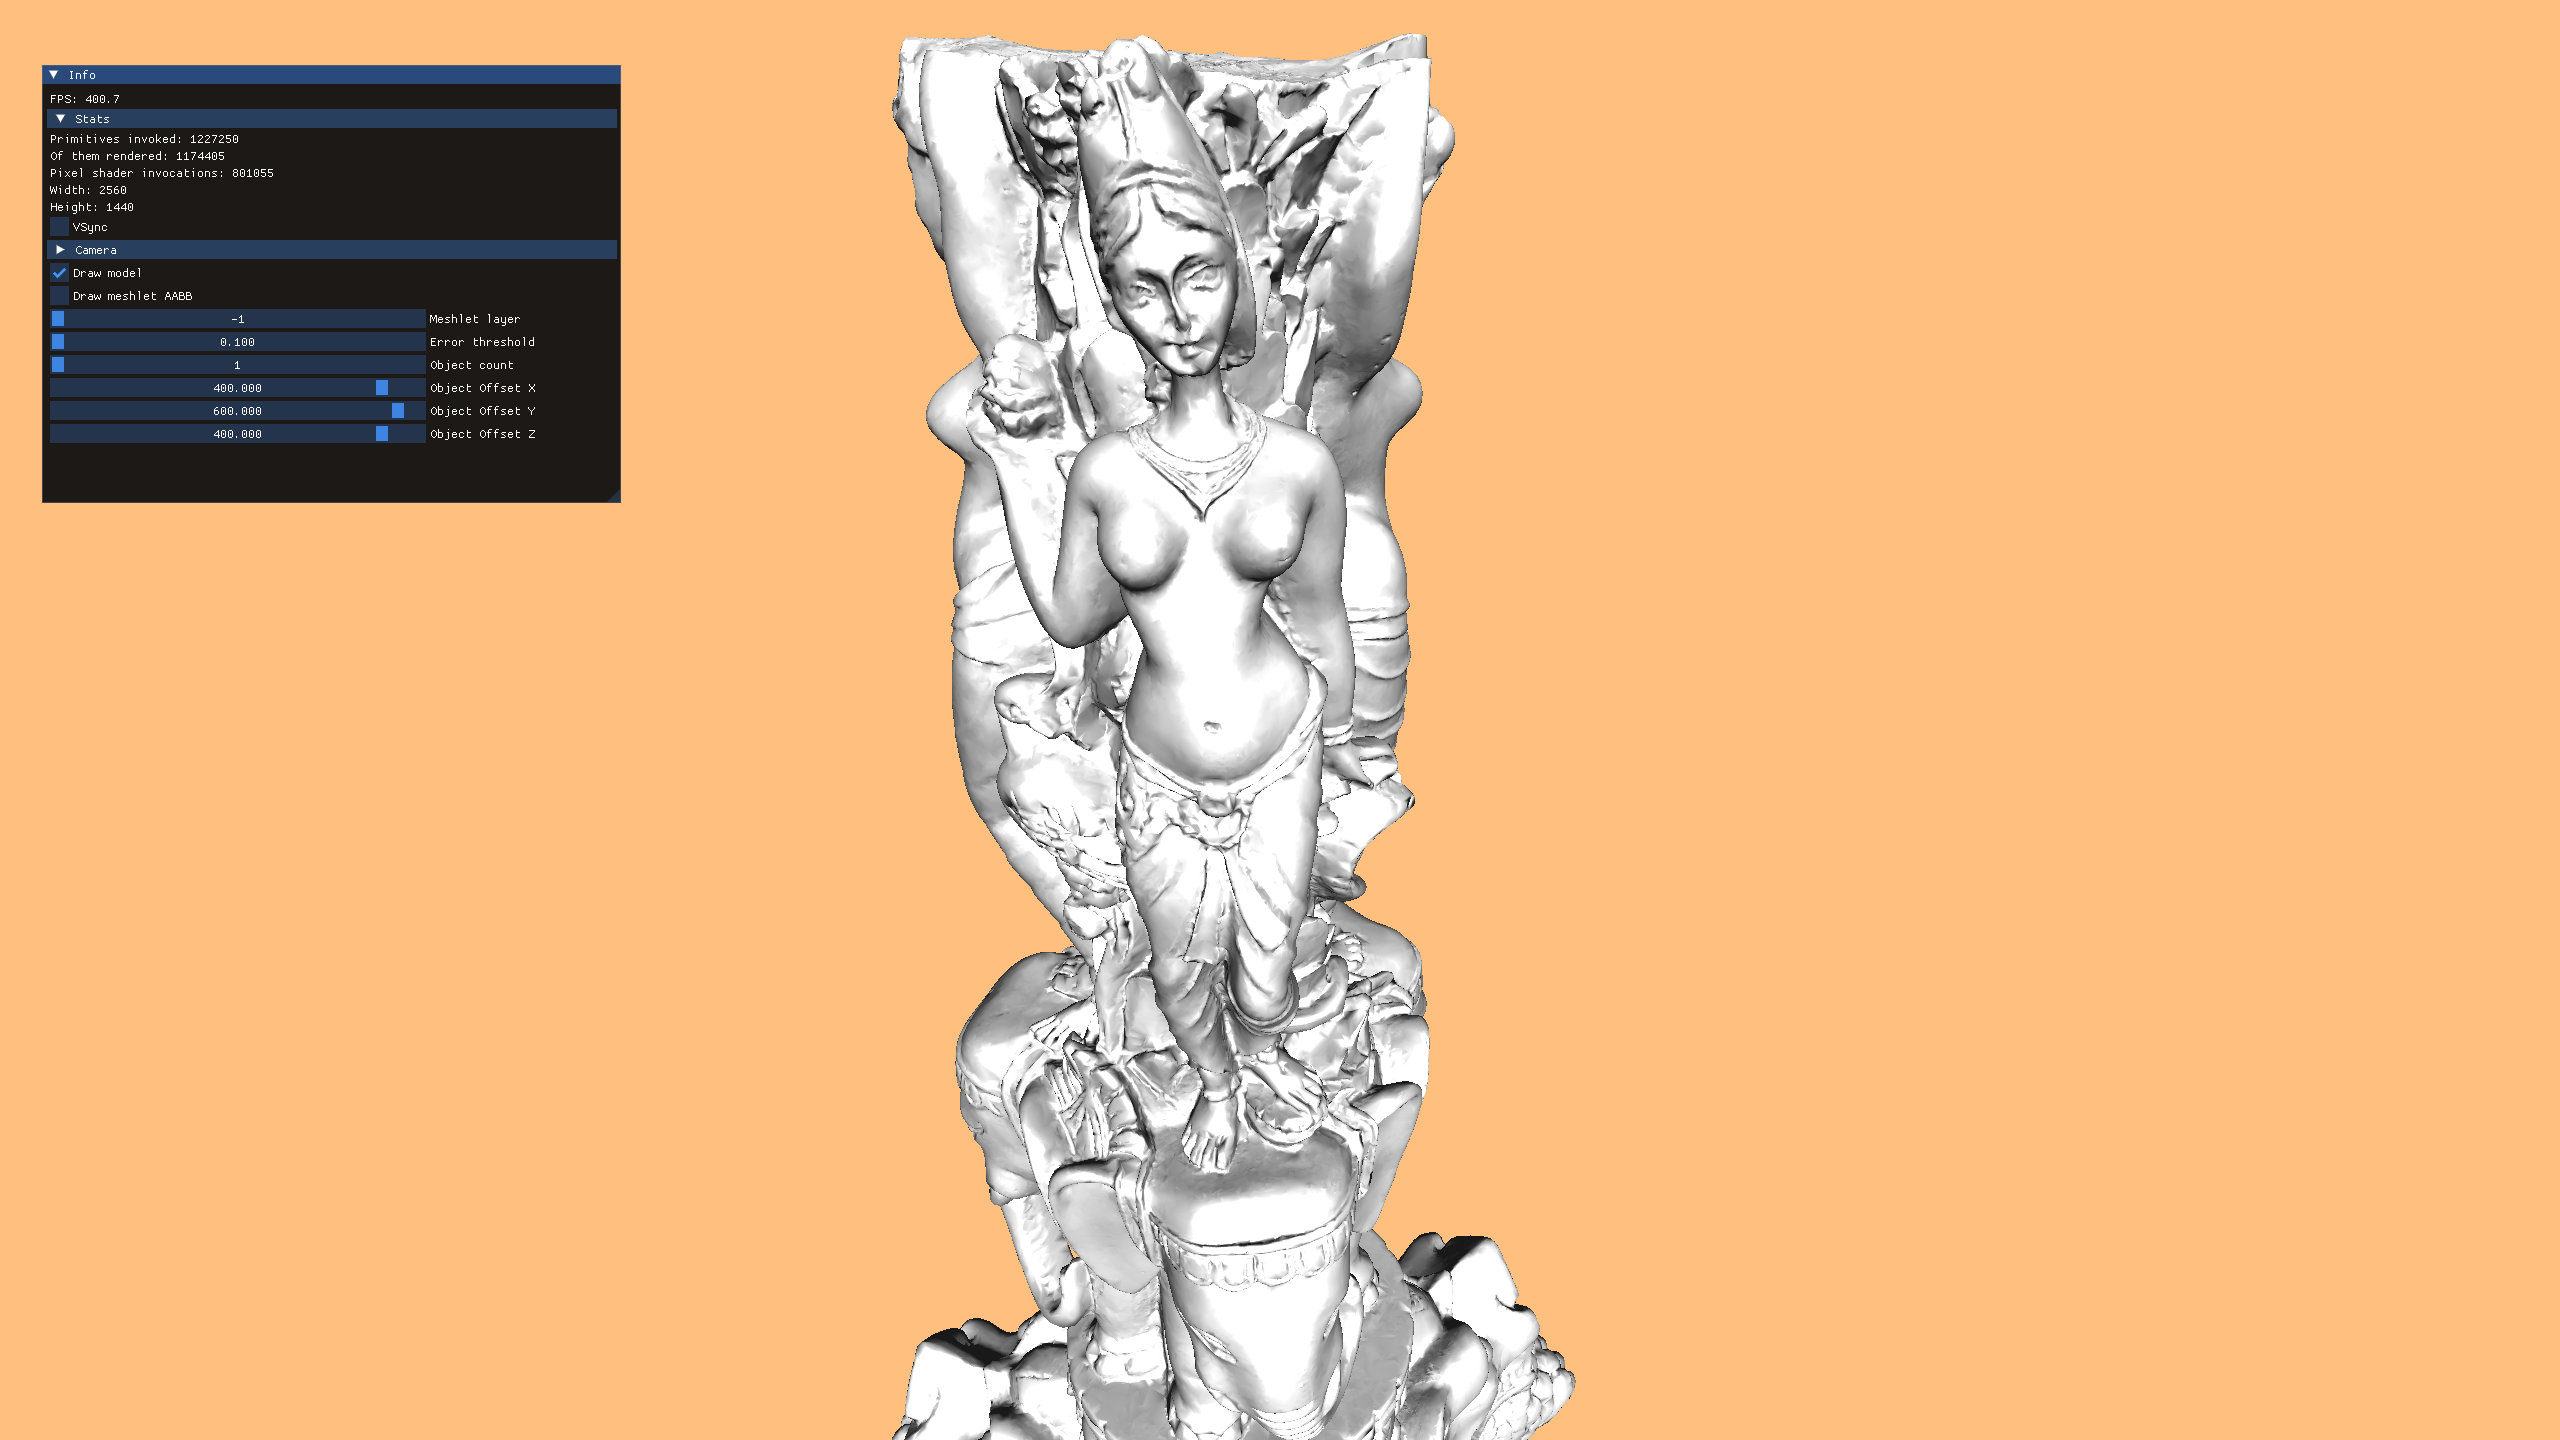
\includegraphics[width=\textwidth]{pics/impl-example-0.png}
    \end{subfigure}
    \begin{subfigure}{.45\textwidth}
        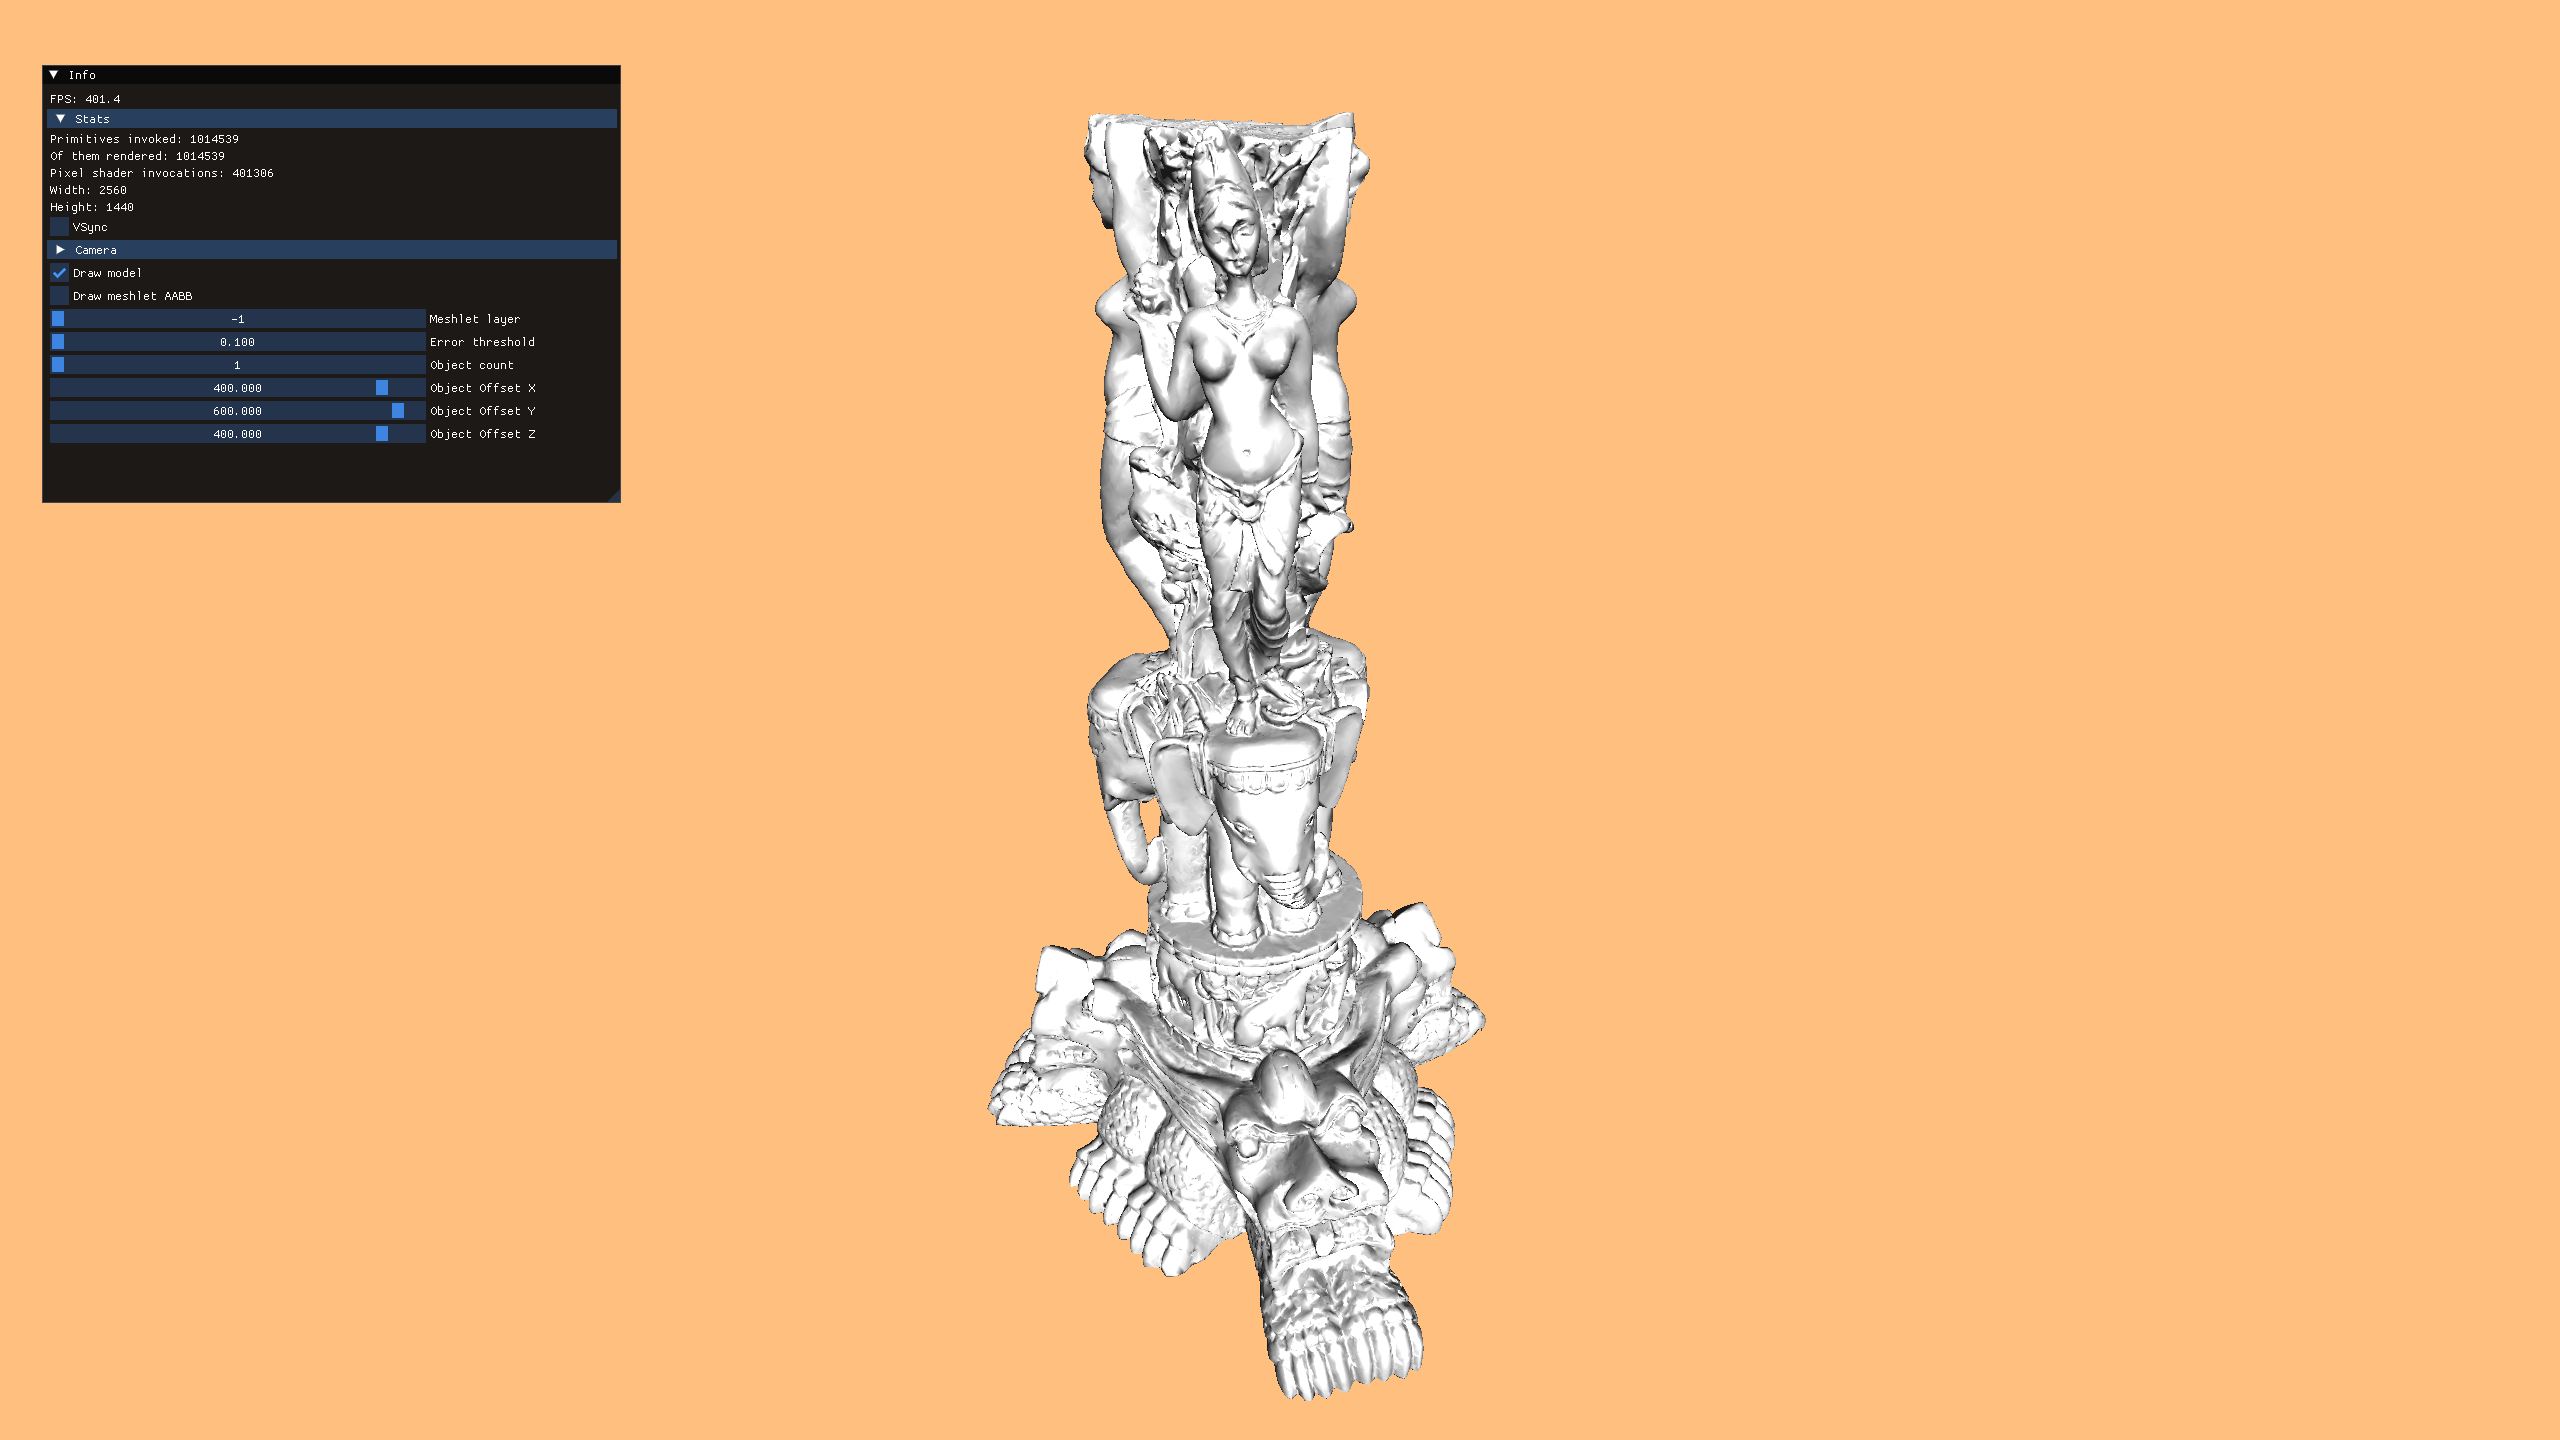
\includegraphics[width=\textwidth]{pics/impl-example-1.png}
    \end{subfigure}

    \medskip

    \begin{subfigure}{.45\textwidth}
        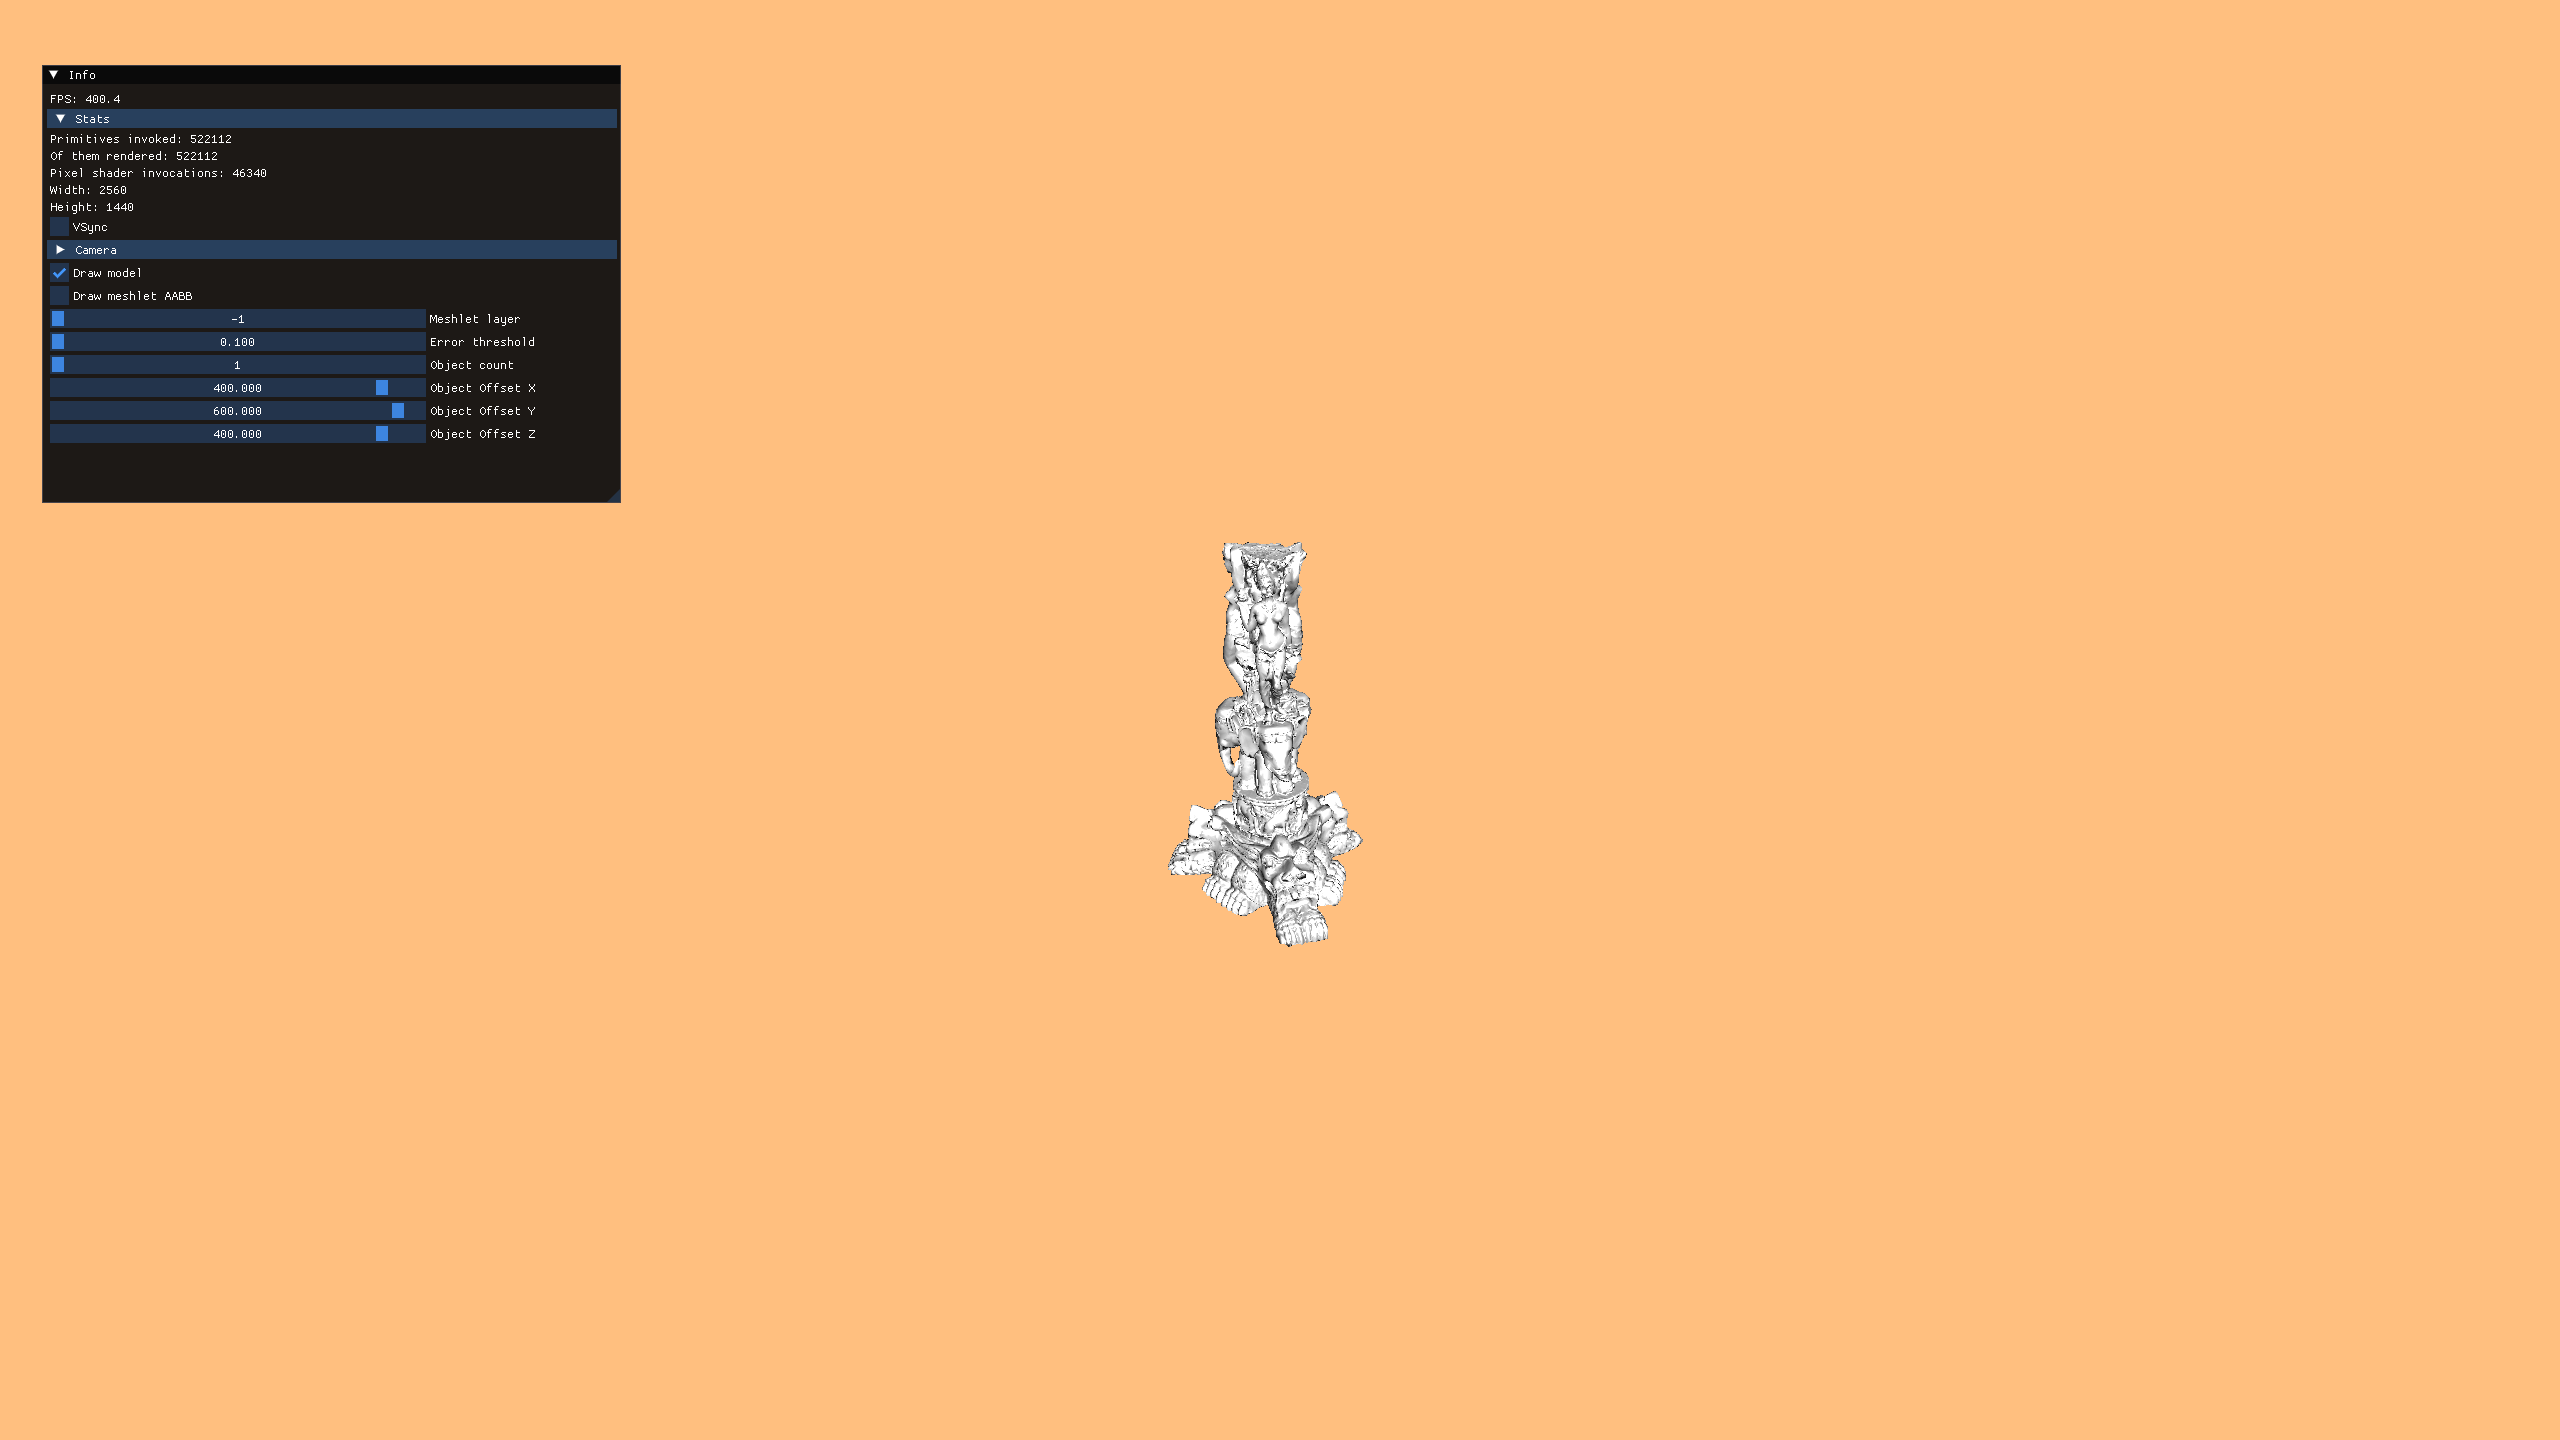
\includegraphics[width=\textwidth]{pics/impl-example-2.png}
    \end{subfigure}
    \begin{subfigure}{.45\textwidth}
        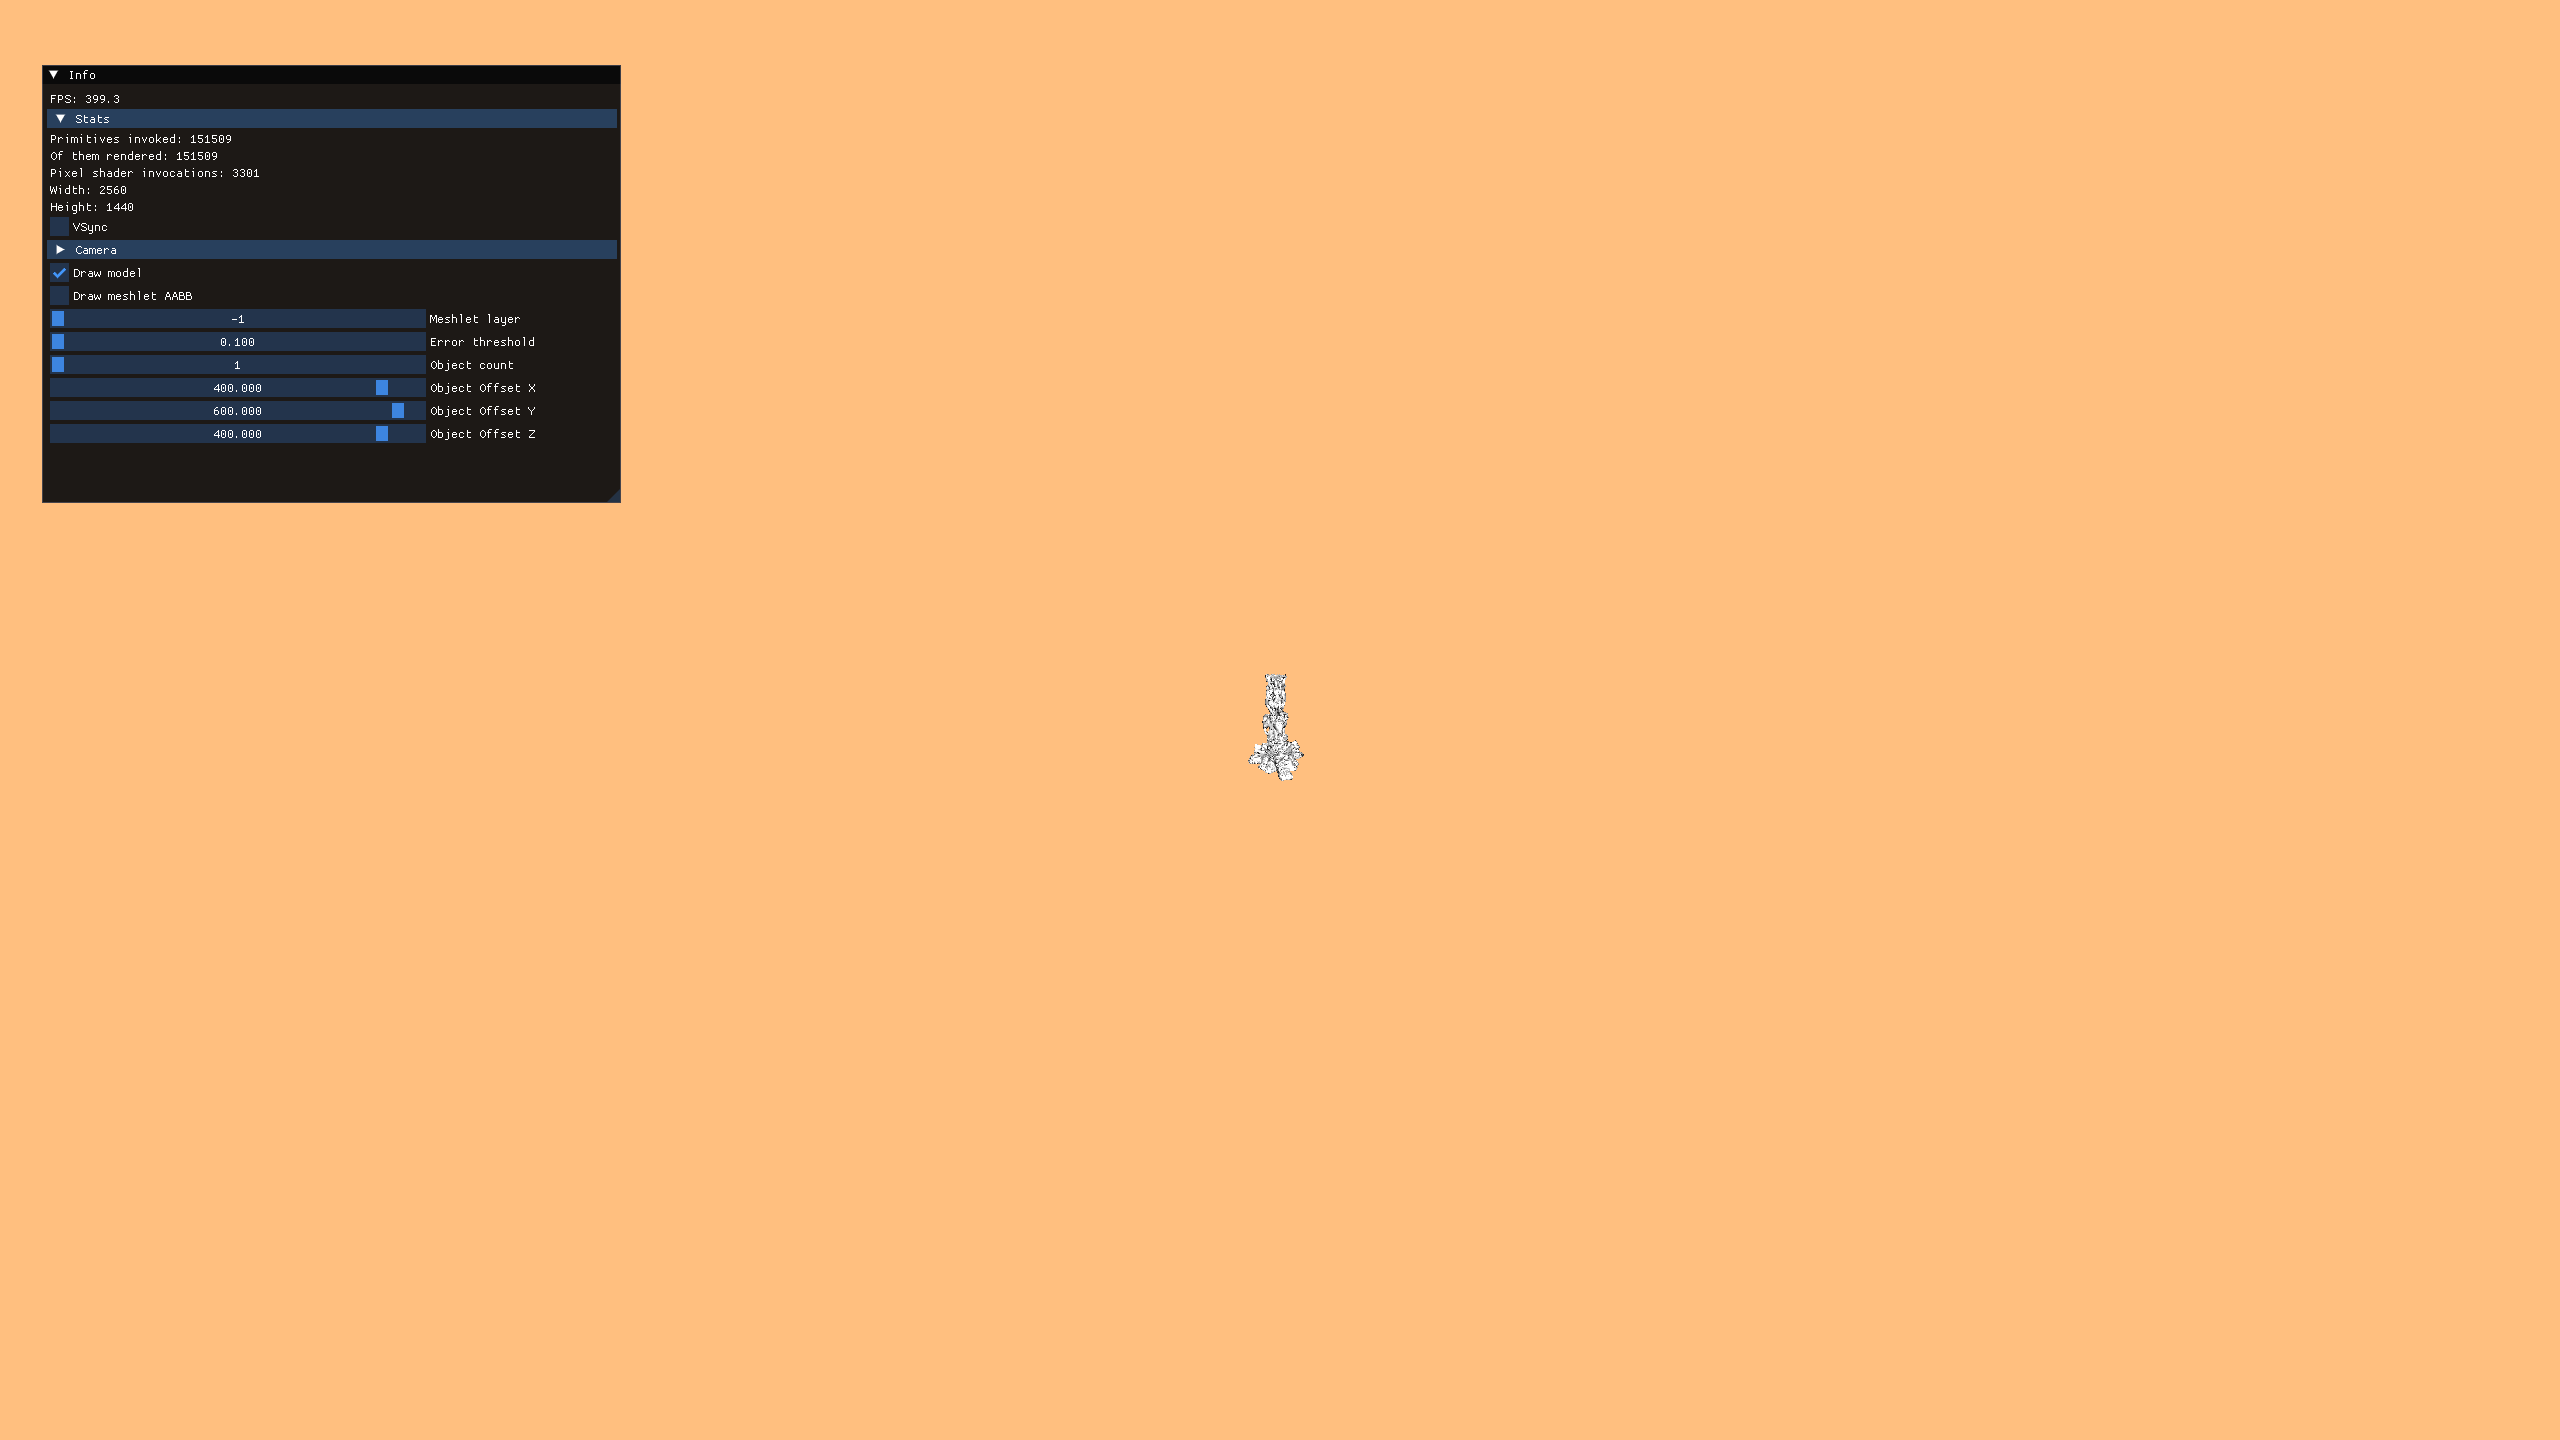
\includegraphics[width=\textwidth]{pics/impl-example-3.png}
    \end{subfigure}
    \caption{Один объект на разных удалениях}
    \label{fig:impl-example}
\end{figure}

\subsection*{Итоги главы}
Таким образом, в главе приведены детали реализации упрощённой системы динамической кластерной детализации.
В ходе реализации были выявлены принципиальные ограничения такой технологии и существенные технические проблемы, которые необходимо решать при реализации полной версии.

    \begin{frame}{Проблемы при реализации}
    В ходе реализации упрощённой системы удалось выделить следующие технические проблемы потребуется решать при реализации полной версии технологии:
    \begin{itemize}
        \item Задача разбиения графа --- NP-трудная\footnote{\url{https://hal.science/hal-00678179/document}}, нужно приближать
        \item Ограничение размера мешлетов
        И в Nanite, и в упрощённой реализации --- приближение
        \item Оптимизация децимации
        \item Оптимизация структуры мешлетов
        --- производительность сильно зависит от количества чтений видеопамяти
        \item Оптимизация отрисовки треугольников
        --- аппаратный растеризатор не рассчитан на треугольники в 1 пиксель, которые нужны кластерной детализации
        \item Организация параллельного спуска по графу
    \end{itemize}
\end{frame}

    \begin{frame}{Принципиальные ограничения}
    \begin{itemize}
        \item Оценка искажения не зависит от направления взгляда
        \item Невозможность анимации меша
        \item Невозможность автоматической децимации некоторых мешей, напр. листвы
        \item Необходимость использовать меши сверхвысокого разрешения, иначе переключения лодов сильно заметны
    \end{itemize}
\end{frame}

% \begin{frame}{Принципиальное ограничение: объём}
%     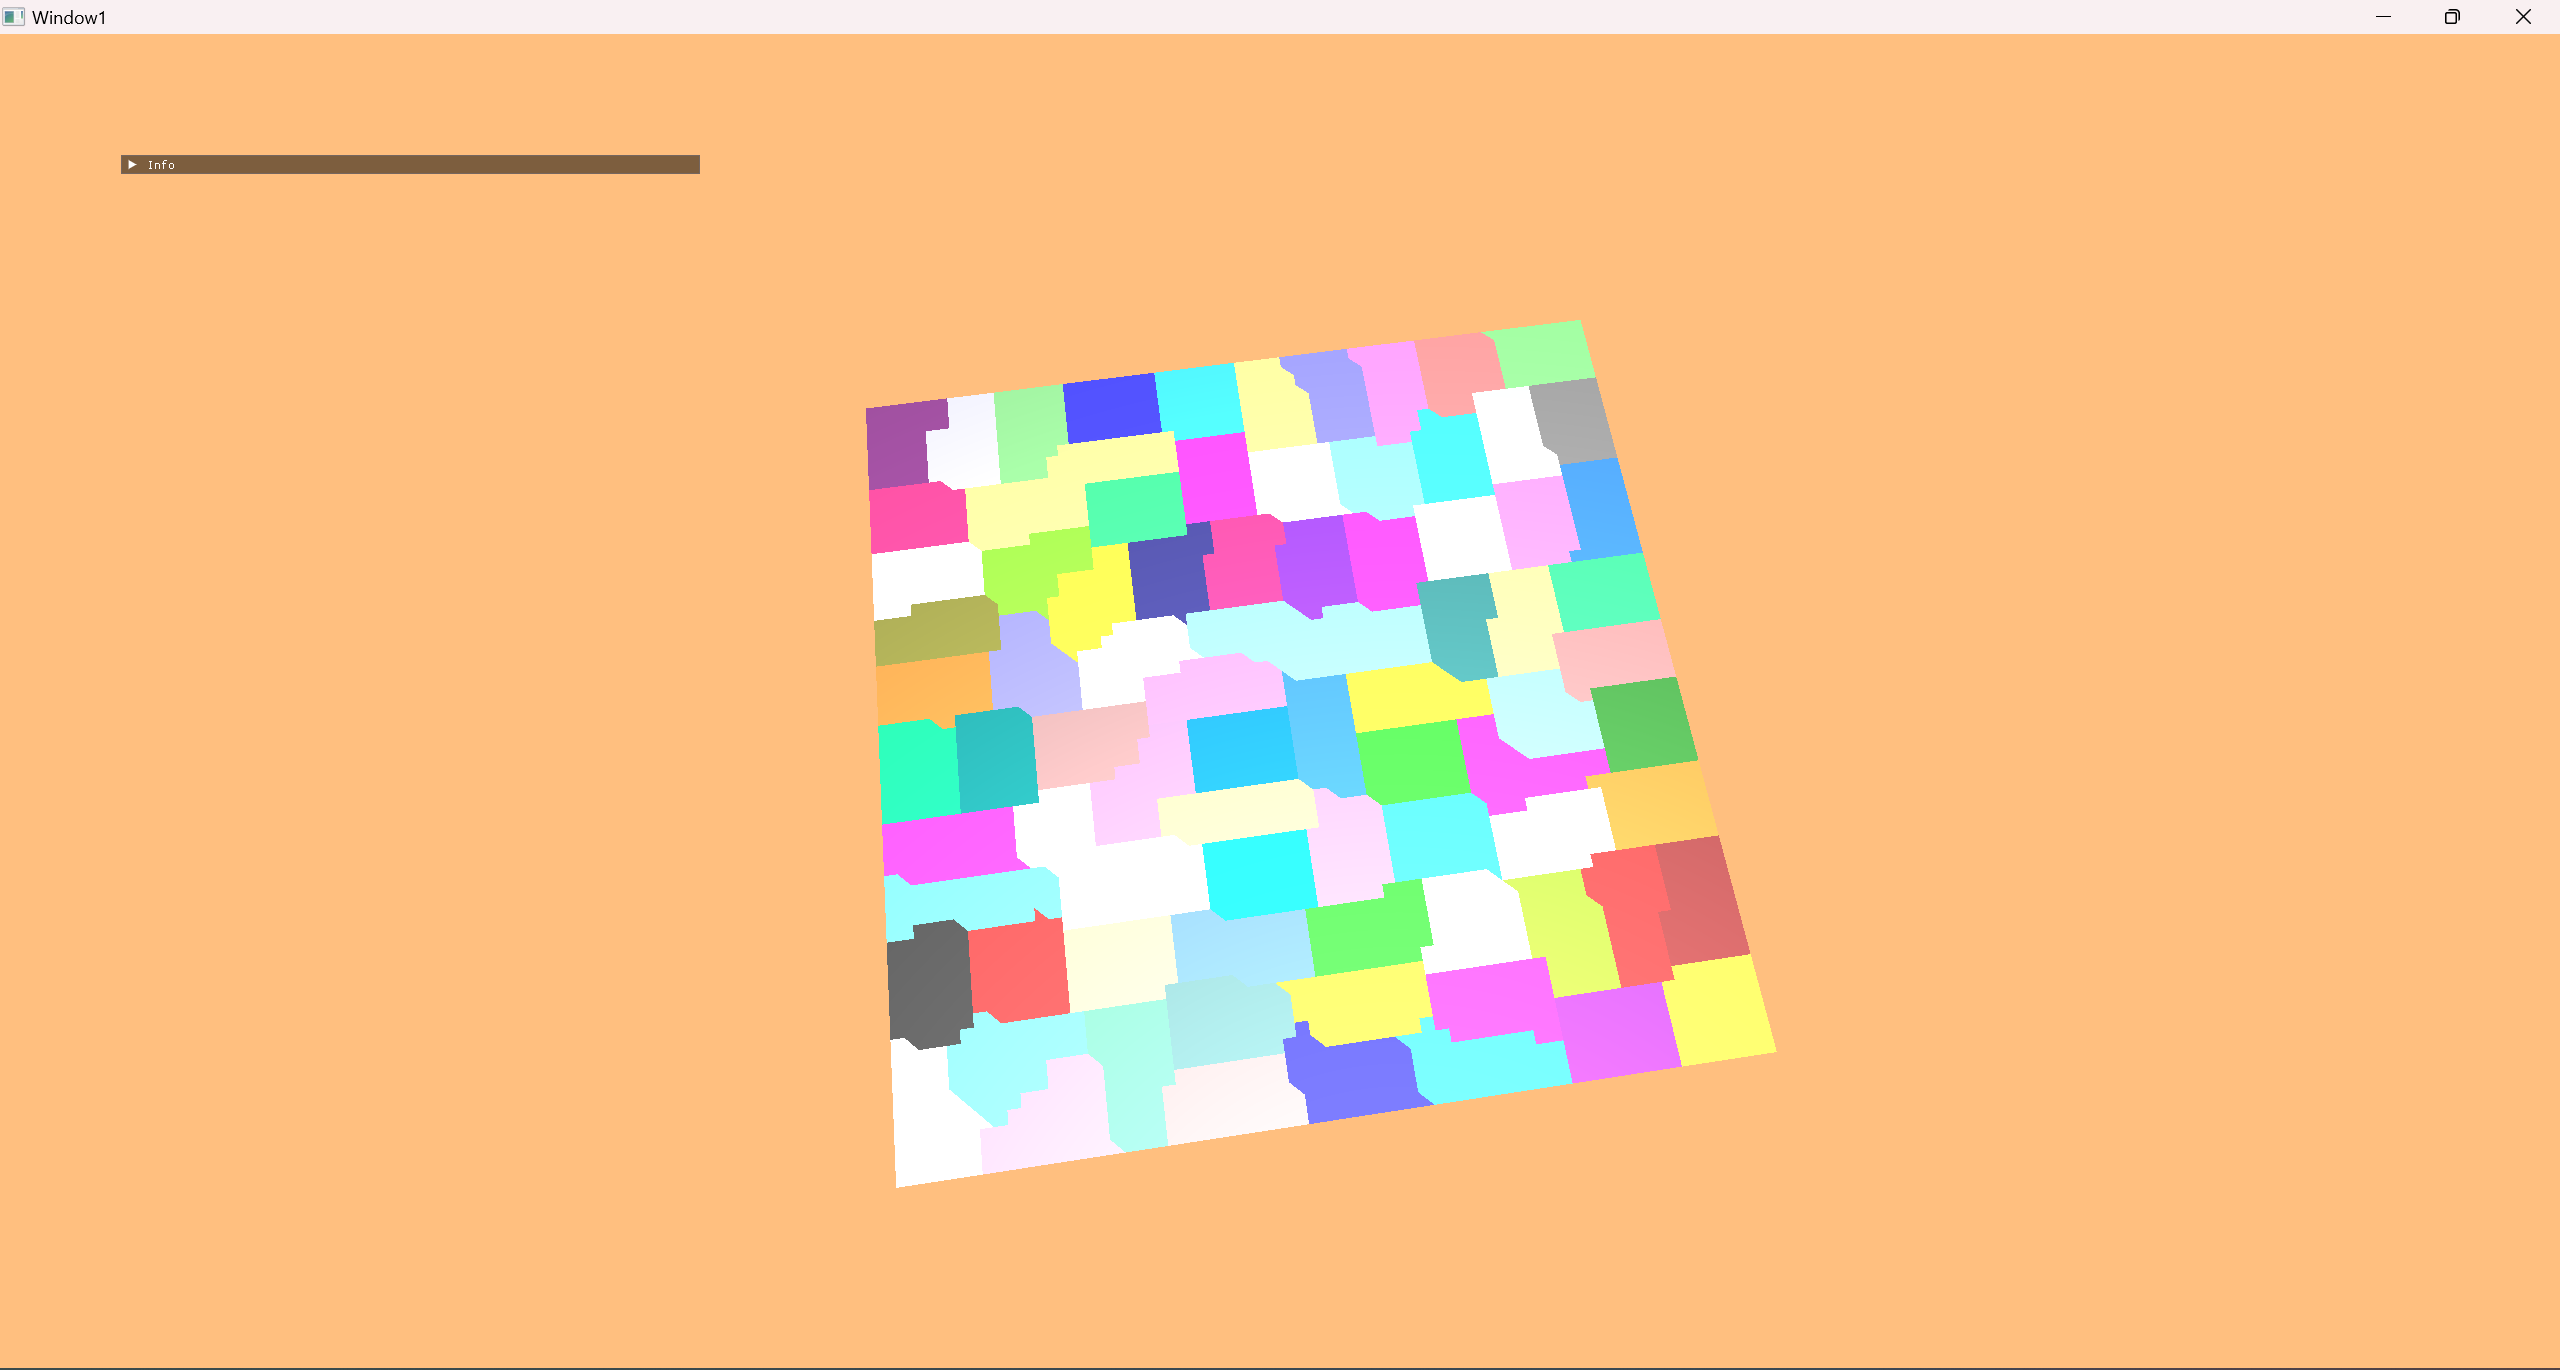
\includegraphics[width=\textwidth]{plane0.png}
% \end{frame}

% \begin{frame}{Принципиальное ограничение: объём}
%     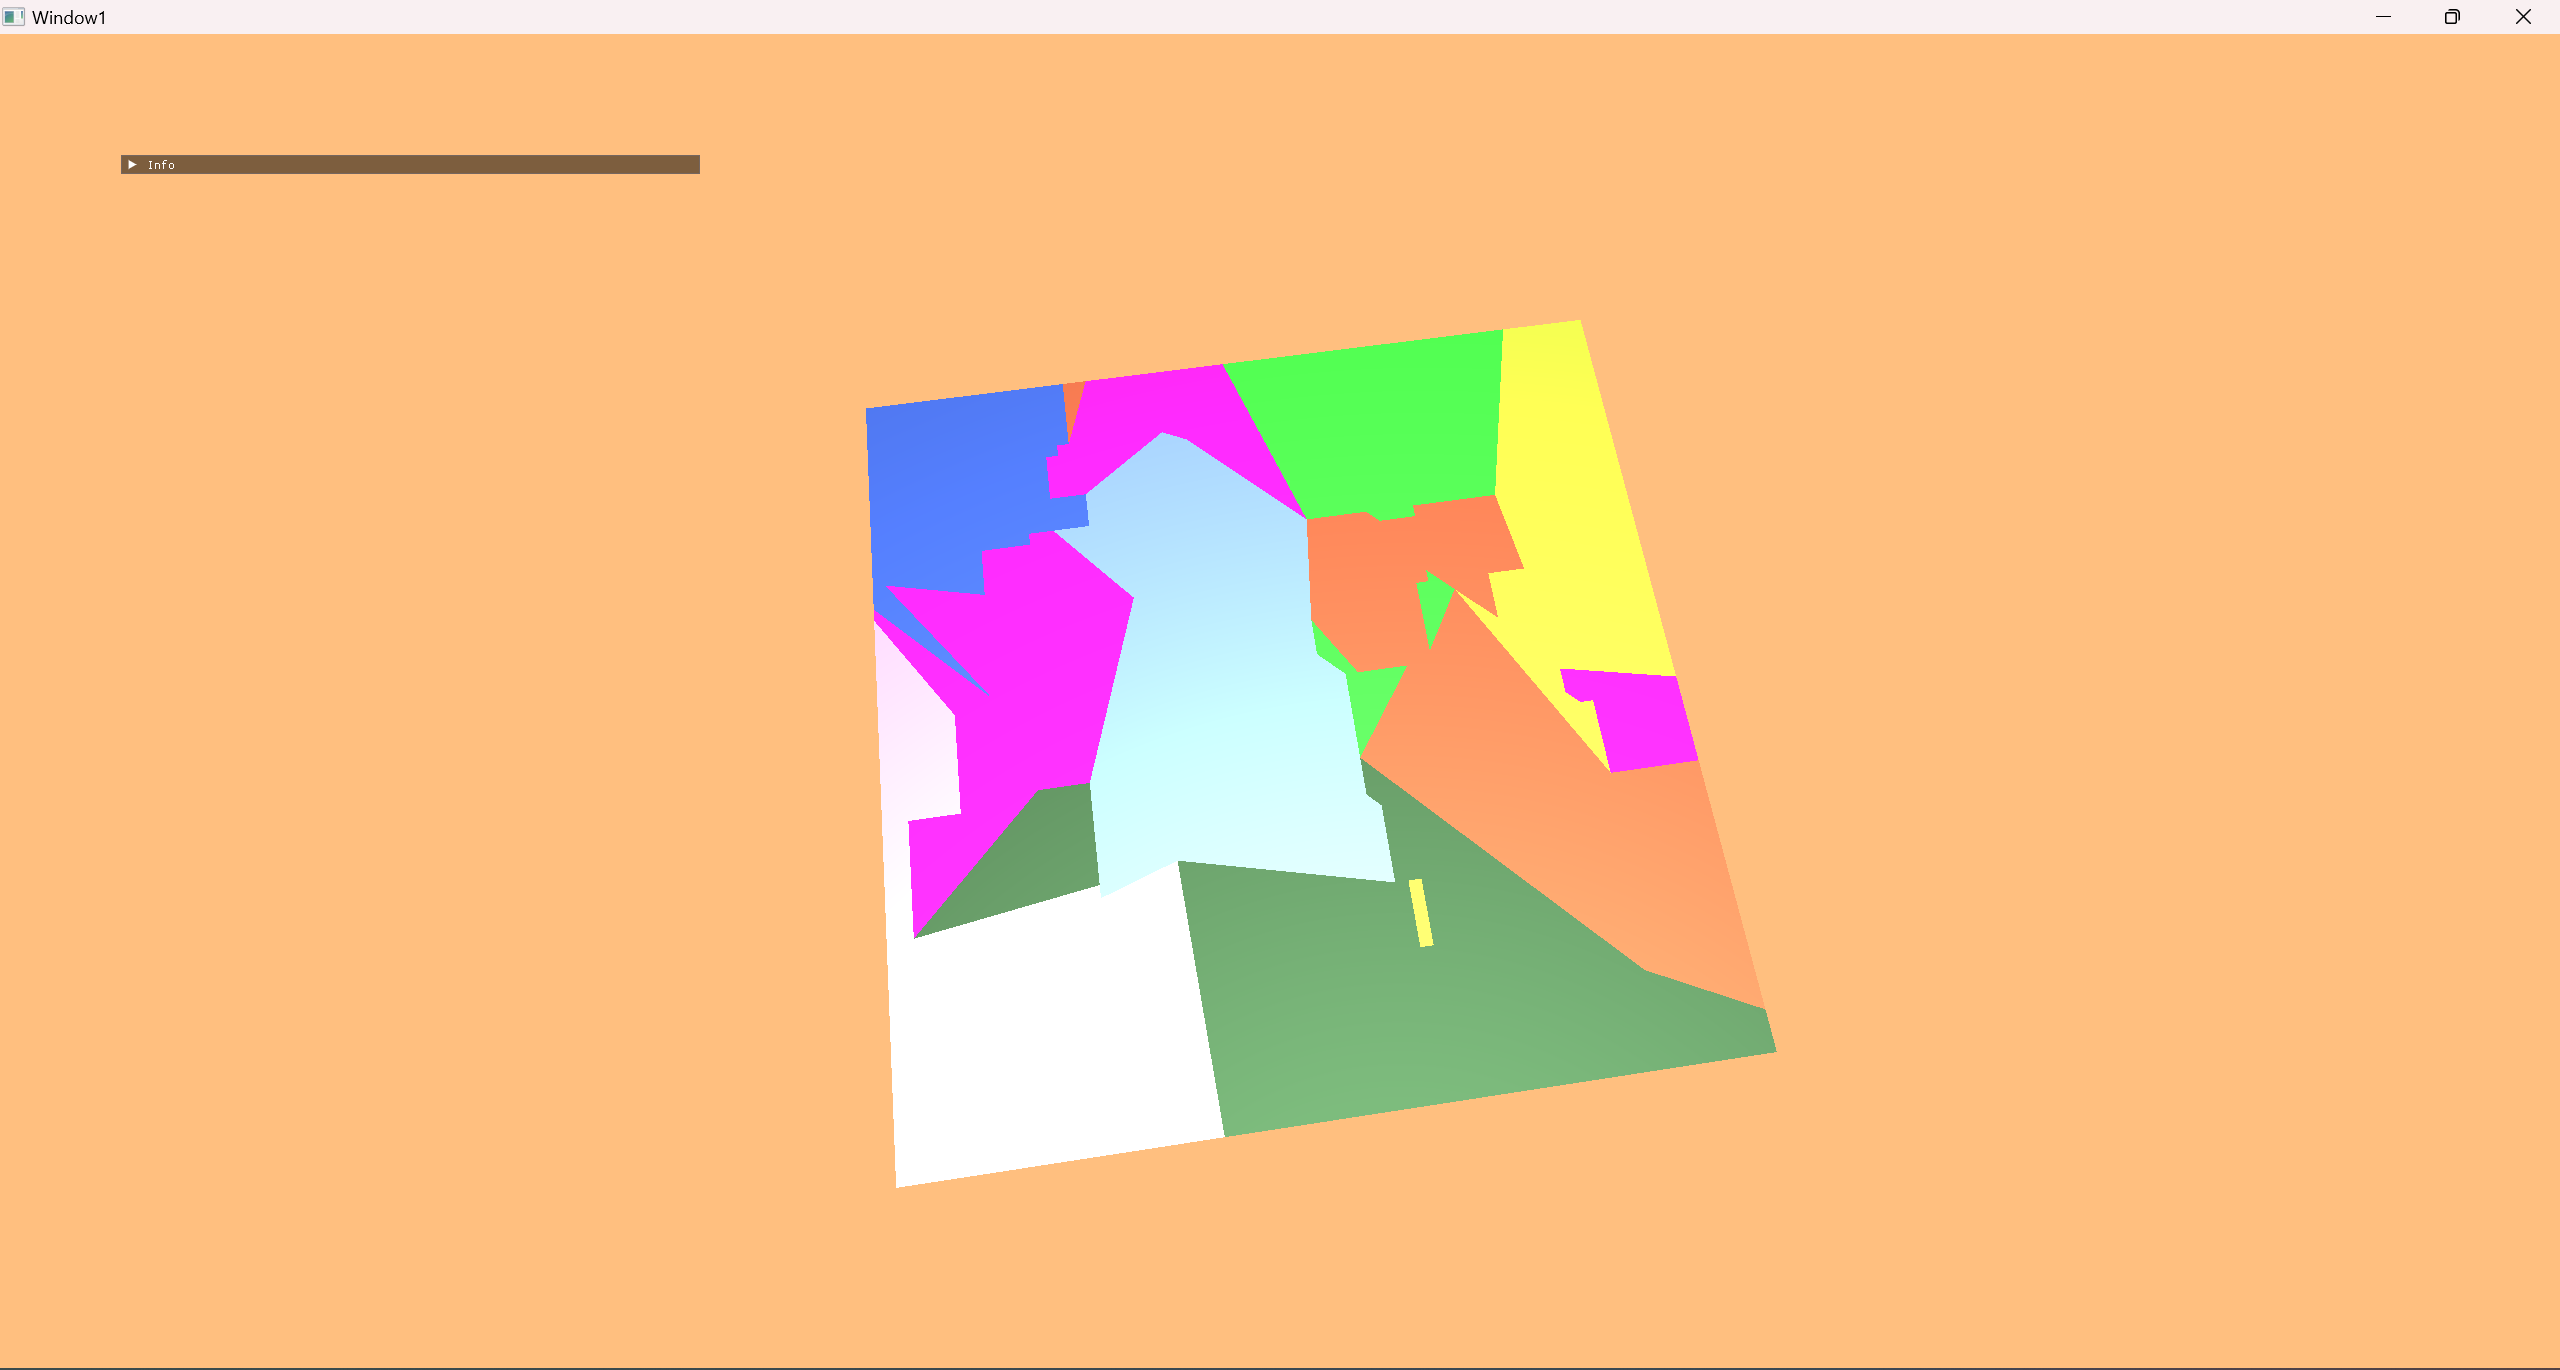
\includegraphics[width=\textwidth]{plane1.png}
% \end{frame}

    \clearpage
\section{5 СРАВНЕНИЕ С КЛАССИЧЕСКОЙ РЕАЛИЗАЦИЕЙ}
TODO

    \begin{frame}{Результаты}
    \begin{itemize}
        \item Продемонстрирована работоспособность технологии
        \item Изучен механизм работы Nanite
        \item Реализована упрощённая версия системы
        \item Определены технические проблемы, которые необходимо решать при реализации полной версии технологии
        \item Определены принципиальные ограничения технологии, её границы применимости
        \item Сравнение с монолитным лоддированием показало, что для внедрения технологии в реальный проект нужны дальнейшие исследования
    \end{itemize}
\end{frame}

    \newcounter{finalframe}
    \setcounter{finalframe}{\value{framenumber}}
    \begin{frame}{Доп.: Geometry Clipmaps}
    \begin{minipage}{.5\textwidth}
        \begin{itemize}
            \item Для ландшафта можно построить растровую карту высот
            \item Уменьшение детализации растровых изображений --- хорошо изученная задача
            \item По карте высот можно без разрывов рисовать геометрию разной детализации
        \end{itemize}
    \end{minipage}
    \begin{minipage}{.45\textwidth}
        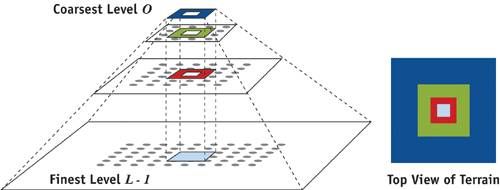
\includegraphics[width=\textwidth]{02_clipmaps_01.jpg}

        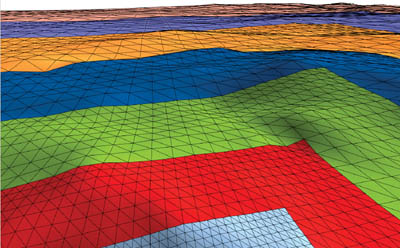
\includegraphics[width=\textwidth]{02_clipmaps_02.jpg}
    \end{minipage}
\end{frame}

\begin{frame}{Доп.: Sparse Voxel Octree}
    \centering
    \begin{minipage}{.75\textwidth}
        \begin{itemize}
            \item Меши приближают поверхность объекта
            \item Можно приближать не поверхность объекта, а его объём
            \item Воксель --- элементарная единица объёма
            \item Приближение объёма вокселями --- фактически, трёхмерное растровое изображение
            \item Одинаковые воксели группируются в кубы для экономии памяти и ускорения вычислений
        \end{itemize}
    \end{minipage}
    \begin{minipage}{.2\textwidth}
        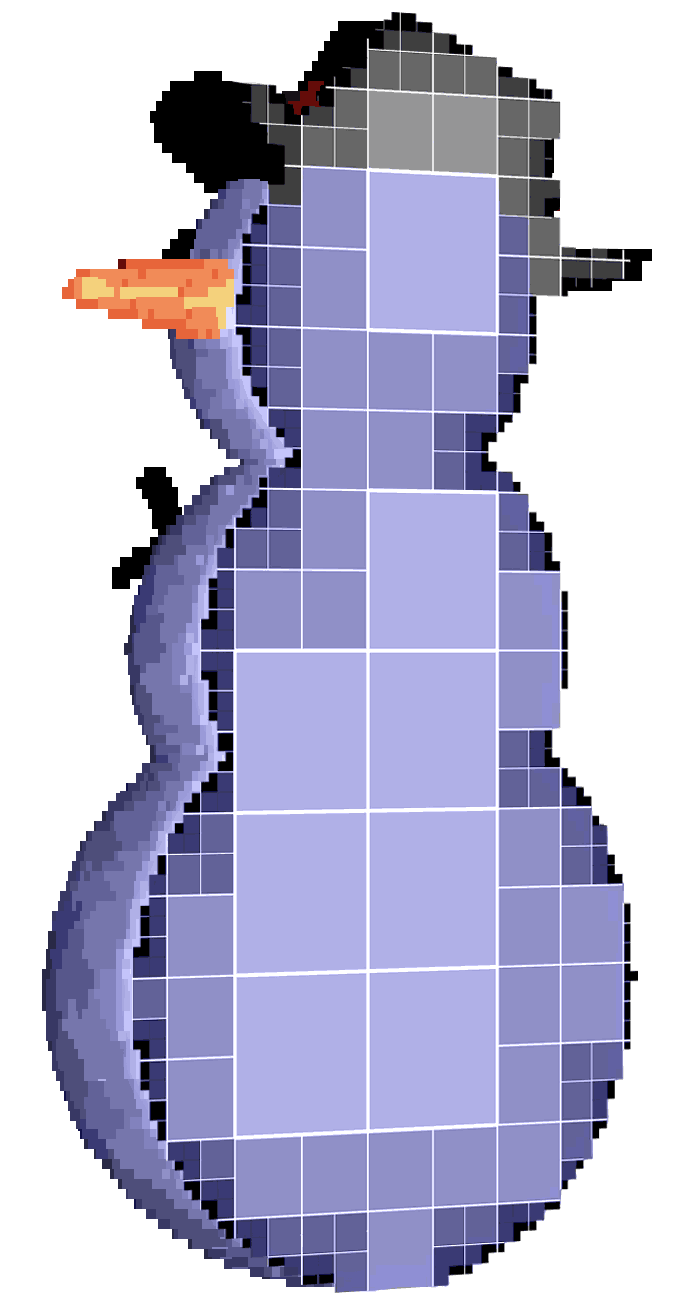
\includegraphics[width=\textwidth]{../Text/pics/SVO-voxel-snowman-slice-01.png}
    \end{minipage}
\end{frame}

\begin{frame}{Доп.: Плотность треугольников}
    \begin{center}
        \includegraphics[width=.45\textwidth]{../Text/pics/heatmap-mono.png}
        \includegraphics[width=.45\textwidth]{../Text/pics/heatmap-cluster.png}
        \includegraphics[width=.45\textwidth]{../Text/pics/heatmap-0.png}
    \end{center}
\end{frame}

    \setcounter{framenumber}{\value{finalframe}}
\end{document}
